\chapter{Fundamentarea teoretică și documentarea bibliografică}
\label{cap:cap2}

Dezvoltarea platformelor moderne pentru gestionarea resurselor hardware distribuite necesită integrarea unor paradigme arhitecturale complexe. Acest capitol prezintă conceptele de Cloud Computing, cu accent pe infrastructura OpenStack, tehnologiile de virtualizare și mecanismele de procesare asincronă. Totodată, sunt analizate soluțiile existente pe piață pentru a identifica limitele actuale și a defini specificațiile tehnice ale platformei propuse.

\section{Concepte și teorii relevante pentru tema abordată}

Proiectarea unei platforme de tip Virtual Private Server (VPS) presupune abstractizarea resurselor fizice și expunerea acestora printr-un nivel de servicii (API), a căror performanță depinde direct de modelul de concurență ales.

\subsection{Cloud Computing și modelul IaaS}

Conform Institutului Național de Standarde și Tehnologie (NIST) \cite{mell2011nist}, modelul \textit{Infrastructure as a Service} (IaaS) reprezintă nivelul de bază al Cloud Computing-ului. Acest model furnizează resurse de calcul, stocare și rețea virtualizate, permițând rularea de sisteme de operare și aplicații arbitrare, clientul având control complet asupra mediului virtualizat.

\subsection{Tehnologii de virtualizare și hipervizoare}

Fundamentul unei arhitecturi IaaS este tehnologia de virtualizare. Virtualizarea permite decuplarea resurselor logice de hardware-ul fizic, facilitând rularea simultană a mai multor sisteme de operare izolate pe o singură mașină gazdă \cite{smith2019cloud}. 

Componenta principală al acestui proces este \textit{Hipervizorul} (sau Virtual Machine Monitor - VMM). În arhitecturile moderne de cloud, se utilizează preponderent hipervizoare de tip Bare-Metal, care rulează direct pe hardware-ul serverului. În ecosistemul Linux și OpenStack, standardul industrial este reprezentat de \textbf{KVM (Kernel-based Virtual Machine)} cuplat cu \textbf{QEMU}. KVM transformă nucleul Linux într-un hipervizor nativ, oferind acces direct la instrucțiunile de virtualizare ale procesoarelor fizice (Intel VT-x sau AMD-V), astfel asigurând o performanță apropiată de cea a rulării pe un mediu nevirtualizat (\textit{near bare-metal performance}).

\subsection{Arhitectura OpenStack}

Infrastructura fizică bazată pe hipervizoare este orchestrată prin intermediul platformei \textbf{OpenStack}, standardul pentru implementările IaaS open-source. Conform documentației oficiale de arhitectură \cite{openstack_architecture}, OpenStack nu este o aplicație monolitică, ci un ecosistem de microservicii decuplate. Fiecare serviciu expune către exterior un API de tip REST și își menține propria bază de date, iar comunicarea internă dintre componentele aceluiași serviciu (de exemplu, între API-ul Nova și agenții de pe nodurile de calcul) se realizează printr-un bus de mesaje (oslo.messaging, de regulă peste RabbitMQ), un model arhitectural similar celui adoptat de platforma dezvoltată în prezenta lucrare. Aplicația interacționează cu următoarele servicii:

\begin{itemize}
    \item \textbf{Keystone (Identity Service):} Funcționează ca serviciu central pentru autentificare și autorizare \cite{openstack_keystone}. Gestionează identitățile utilizatorilor, permisiunile (pe bază de roluri) și expune un catalog de endpoint-uri (\textit{service catalog}). Keystone este esențial pentru securitatea și descoperirea reciprocă a tuturor celorlalte module OpenStack.
    \item \textbf{Nova (Compute Service):} Componenta principală responsabilă de orchestrarea resurselor de calcul \cite{openstack_nova}. Nova gestionează ciclul de viață al instanțelor și rutează cererile către hipervizoarele KVM/QEMU pentru alocarea resurselor CPU și RAM.
    \item \textbf{Neutron (Networking Service):} Furnizează capabilități de rețelistică bazate pe tehnologii SDN (Software-Defined Networking) \cite{openstack_neutron}. Neutron gestionează crearea de rețele virtuale, subrețele, rutare L3 și alocarea dinamică a adreselor IP.
    \item \textbf{Glance (Image Service):} Acționează ca un registru pentru imaginile mașinilor virtuale \cite{openstack_glance}. Stochează și furnizează șabloanele sistemelor de operare utilizate de Nova în faza de provizionare.
    \item \textbf{Cinder (Block Storage Service):} Oferă volume de stocare persistentă la nivel de bloc \cite{openstack_cinder}, atașate instanțelor compute pentru a asigura persistența datelor dincolo de ciclul de viață volatil al mașinii virtuale.
\end{itemize}

Colaborarea acestor servicii în procesul de creare a unei instanțe este ilustrată în diagrama de arhitectură (Figura \ref{fig:arhitectura_openstack}).

\begin{figure}[H]
    \centering
    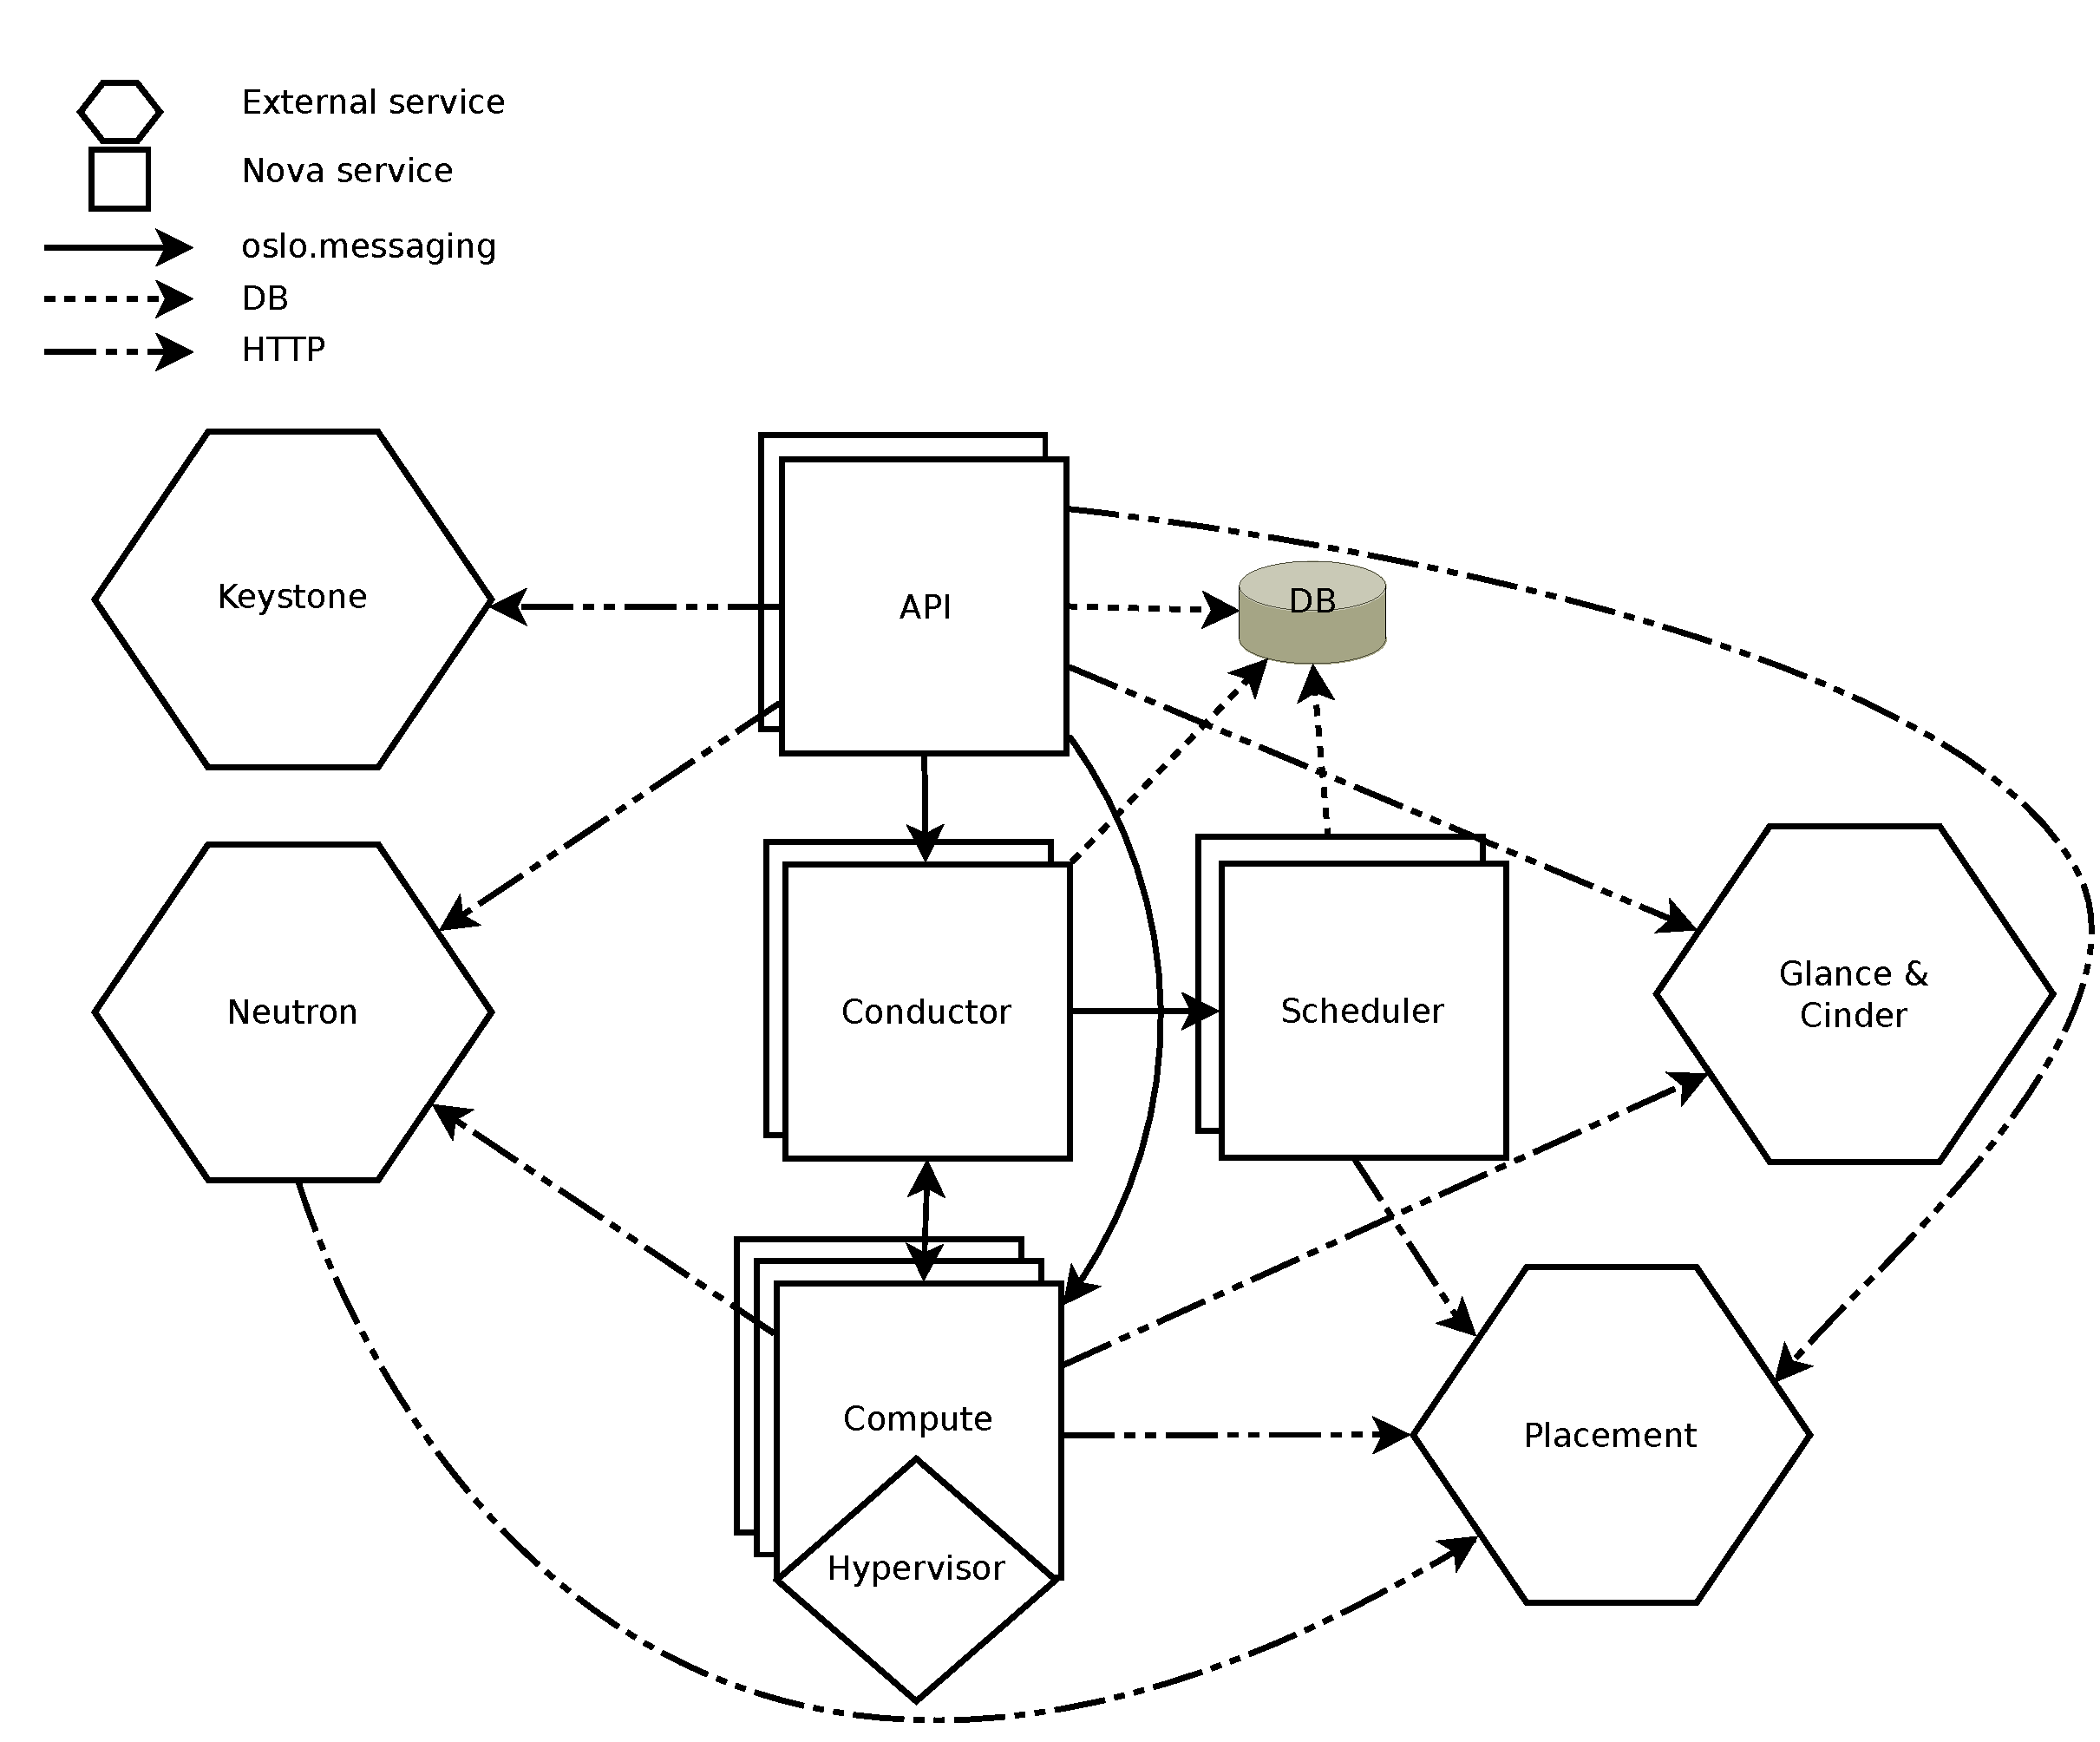
\includegraphics[width=0.95\textwidth]{continut/capitol2/figuri/architecture.pdf}
    \caption{Interacțiunea componentelor arhitecturale OpenStack utilizate în procesul de provizionare \cite{openstack_nova}.}
    \label{fig:arhitectura_openstack}
\end{figure}

Deoarece platforma propusă este construită utilizând aceste servicii, este necesară o prezentare detaliată a mecanismelor lor interne, a modelului de implementare și a limitărilor pe care le impun, aspecte tratate în subsecțiunile următoare.

\subsubsection{Modelul de implementare și împachetarea serviciilor}

Instalarea manuală componentelor OpenStack și gestionarea dependențelor dintre acestea reprezintă un proces complicat și predispus la erori. Din acest motiv, implementarea propusă utilizează \textbf{Kolla-Ansible} \cite{openstack_kolla}, o metodă de desfășurare care împachetează fiecare serviciu OpenStack într-un container Docker dedicat și automatizează configurarea și orchestrarea acestora prin intermediul unor playbook-uri Ansible. Containerizarea izolează dependențele fiecărui serviciu, asigură reproductibilitatea mediului și simplifică operațiunile de actualizare.

Mediul a fost configurat în regim \textit{all-in-one}, în care planul de control (API-urile serviciilor, planificatorul, bazele de date interne și brokerul de mesaje) și planul de calcul (hipervizorul care găzduiește mașinile virtuale) se află pe un singur nod. Această topologie reduce semnificativ cerințele hardware și este adecvată unui mediu educațional sau de dezvoltare, însă prezintă două limitări: capacitatea totală a sistemului este restrânsă la resursele unui singur nod, iar absența redundanței (lipsa unei configurații de tip \textit{High Availability}) face ca o defecțiune a nodului să afecteze întreaga platformă. Aceste constrângeri sunt analizate în capitolul dedicat testării.

\subsubsection{Serviciul de calcul Nova și planificarea resurselor}

Nova reprezintă componenta centrală responsabilă de gestionarea ciclului de viață al mașinilor virtuale. O instanță este definită prin combinația dintre o imagine (sistemul de operare) și un \textbf{flavor} - un șablon care fixează cantitatea de resurse virtuale alocate: numărul de procesoare virtuale (vCPU), cantitatea de memorie RAM și dimensiunea discului rădăcină.

La primirea unei cereri de creare, Nova nu alege arbitrar nodul pe care va rula instanța, ci deleagă această decizie serviciului \textbf{Placement} \cite{openstack_placement} și unui planificator de tip filtru (\textit{Filter Scheduler}), care selectează un nod de calcul ce dispune de resurse suficiente. În cazul în care niciun nod nu poate satisface cererea, planificatorul returnează eroarea \texttt{NoValidHost}, iar instanța trece în starea \texttt{ERROR}. Un aspect important pentru înțelegerea limitelor de capacitate ale platformei îl reprezintă supraalocarea (\textit{overcommit}): în mod implicit, Nova permite alocarea unui număr de procesoare virtuale de până la șaisprezece ori mai mare decât numărul de nuclee fizice și a unei cantități de memorie de 1,5 ori mai mare decât cea fizică, pornind de la premisa potrivit căreia instanțele nu își utilizează simultan întreaga capacitate. În consecință, factorul care limitează în practică numărul de mașini virtuale ce pot fi create este, de regulă, memoria RAM sau spațiul de stocare, și nu numărul de procesoare.

Nova traduce cererile abstracte în operațiuni concrete prin intermediul bibliotecii \textbf{libvirt}, care controlează hipervizorul \textbf{KVM/QEMU} \cite{linux_kvm}, astfel asigurând crearea resurselor virtuale pe hardware-ul fizic.

\subsubsection{Rețelistica definită software prin Neutron}

Neutron implementează un model de rețelistică definită software (SDN), construit pe arhitectura de tip plugin \textbf{ML2 (Modular Layer 2)}, care decuplează modelul logic al rețelei de tehnologia concretă de comutare (în mod uzual, agentul Open vSwitch). Platforma propusă adoptă un model de rețea de tip \textit{VPC} (\textit{Virtual Private Cloud}): fiecare organizație dispune de rețele private izolate (\textit{tenant networks}), împărțite în subrețele și conectate la exterior printr-un \textbf{ruter virtual} gestionat de agentul L3.

Accesul public la instanțe este realizat prin \textbf{adrese IP flotante (\textit{floating IPs})}, alocate dintr-un bazin de adrese al rețelei externe și asociate dinamic instanțelor prin translatare de adrese (NAT) - un model echivalent conceptual cu adresele IP elastice (\textit{Elastic IP}) din Amazon EC2. Filtrarea traficului la nivelul fiecărei instanțe se realizează prin \textbf{grupuri de securitate (\textit{security groups})}, care funcționează ca firewall-uri cu stare (\textit{stateful}) aplicate direct asupra porturilor virtuale, ce permit definirea granulară a regulilor de acces de intrare și de ieșire.

\subsubsection{Gestiunea imaginilor (Glance) și a stocării bloc (Cinder)}

Glance funcționează ca un registru centralizat pentru șabloanele sistemelor de operare, stocate de regulă în format \texttt{qcow2} (format care suportă alocarea leneșă a spațiului - \textit{thin provisioning}) sau \texttt{raw}. Pentru importul imaginilor personalizate, platforma exploatează metoda \textit{web-download}, prin care Glance descarcă fișierul imaginii direct de la un URL specificat, evitând astfel transferul fișierelor de dimensiuni mari prin backend-ul platformei dezvoltate.

Cinder oferă stocare persistentă la nivel de bloc, expusă instanțelor sub forma unor volume independente. Implementarea utilizează driver-ul \textbf{LVM (\textit{Logical Volume Manager})}, care alocă volumele dintr-un grup de volume fizice. Distincția fundamentală se face între discul \textbf{efemer} (alocat din spațiul local al nodului de calcul și distrus odată cu ștergerea instanței) și volumul \textbf{persistent} oferit de Cinder. Platforma utilizează ambele moduri de operare: o instanță poate porni fie de pe discul efemer definit de flavor, fie direct de pe un volum Cinder (\textit{boot-from-volume}), în acest caz root disk-ul supraviețuiește ștergerii mașinii virtuale și poate fi reutilizat.

\subsubsection{Identitate și autorizare prin Keystone}

Keystone reprezintă punctul central de autentificare și autorizare al întregului ecosistem. Modelul său de date organizează utilizatorii în \textbf{proiecte} (\textit{projects} sau \textit{tenants}) și domenii, cărora le sunt asociate roluri ce determină permisiunile. Autentificarea se realizează prin emiterea de token-uri (tip Fernet), pe care celelalte servicii le validează la fiecare cerere. Keystone expune \textbf{catalogul de servicii} (\textit{service catalog}), un registru al adreselor (\textit{endpoint}-urilor) tuturor componentelor, care permite descoperirea reciprocă a serviciilor în cadrul cluster-ului. În implementarea curentă, izolarea dintre organizațiile platformei este realizată la nivelul aplicației (prin filtrarea datelor după identificatorul organizației), toate resursele fiind create în cadrul unui singur proiect OpenStack - o decizie de proiectare discutată în următoarele capitole.

\subsubsection{API REST și versionarea prin microversiuni}

Toate serviciile OpenStack expun funcționalitatea prin API-uri de tip REST. Pentru a evita interacțiunea directă cu aceste endpoint-uri HTTP, platforma utilizează biblioteca \textbf{OpenStack SDK} \cite{openstack_sdk}, care abstractizează autentificarea, gestiunea token-urilor și apelurile către servicii. Un aspect particular al API-ului de calcul îl reprezintă \textbf{versionarea prin microversiuni (\textit{microversions})} \cite{openstack_microversions}: API-ul evoluează incremental, fiecare modificare cu impact asupra compatibilității fiind asociată unei microversiuni distincte, pe care clientul o poate solicita în mod explicit. Acest mecanism asigură compatibilitatea retroactivă, dar necesită mai multă atenție în cadrul implementării, anumite câmpuri (de exemplu, datele agregate privind capacitatea hipervizoarelor) au fost modificate în versiunile recente, fiind necesară stabilirea explicită a unei microversiuni pentru obținerea informațiilor dorite.

\subsection{Procesarea asincronă și tiparele de mesagerie (AMQP)}

Comunicarea cu serviciile OpenStack se realizează utilizând modelul arhitectural REST (\textit{Representational State Transfer}) \cite{fielding2000rest}. Principiul de bază impune ca interacțiunile să fie \textit{stateless}. 

Totuși, provizionarea resurselor IaaS este o operațiune intensivă din punct de vedere al operațiilor de intrare/ieșire și de lungă durată (\textit{long-running operation}). Apelarea sincronă a API-ului OpenStack prezintă limitări severe: firul de execuție al serverului web rămâne blocat așteptând răspunsul infrastructurii, ce conduce la epuizarea rapidă a resurselor serverului web sub un trafic concurent \cite{hohpe2004enterprise}.

Pentru a asigura scalabilitatea, s-a implementat o arhitectură orientată pe mesaje (\textit{Message-Oriented Middleware}). Această abordare decuplează preluarea cererii de execuția propriu-zisă prin intermediul protocolului \textbf{AMQP (Advanced Message Queuing Protocol)}. În cadrul soluției propuse, API-ul (FastAPI) acționează ca un \textit{Publisher}. Cererea HTTP este serializată și trimisă către un broker de mesaje (\textbf{RabbitMQ}). Brokerul o include într-o coadă (\textit{queue}), iar clientul va primi în acest moment un răspuns instantaneu de succes (\texttt{HTTP 202 Accepted}). Ulterior, procesele de fundal (\textit{Consumers} / Worker-ii \textbf{Celery}) extrag mesajele din coadă și inițiază apelurile către OpenStack.

\subsection{Gestiunea datelor și telemetria}

O platformă VPS are nevoie de mai multe tipuri distincte de persistență a datelor. Pentru gestionarea stării sistemului (utilizatori, parole, detalii despre instanțe, statusuri), este necesară o \textbf{bază de date relațională (RDBMS)} compatibilă cu proprietățile ACID (Atomicity, Consistency, Isolation, Durability) \cite{elmasri2015fundamentals}. În acest sens, platforma folosește \textbf{MariaDB}.

În contrast, monitorizarea performanței mașinilor virtuale (telemetria pentru consumul de CPU și RAM) generează cantități mari de date secvențiale, marcate temporal (\textit{timestamps}). Stocarea acestora într-o bază de date relațională ar duce la degradarea rapidă a performanței. Pentru aceste sarcini este necesară utilizarea unei baze de date specializate de tip \textbf{Time-Series (TSDB)}, cum ar fi \textbf{InfluxDB}. Acest tip de baze de date este optimizat nativ pentru stocarea rapidă a metricilor continue și agregarea lor pe intervale de timp, facilitând afișarea în timp real a graficelor de consum în interfața grafică.

\subsection{Bootstrapping și Cloud-init}

Pentru a livra instanțe preconfigurate și complet funcționale, platformele cloud moderne folosesc mecanisme de \textit{bootstrapping}. Standardul industrial pentru inițializarea instanțelor de cloud este \textbf{Cloud-init} \cite{cloudinit_docs}. Acesta este un pachet software instalat în imaginile sistemelor de operare, care rulează la prima pornire a mașinii virtuale. 

Prin intermediul componentelor OpenStack (în special serviciul de Metadata furnizat de Nova), aplicația propusă poate injecta un script de configurare (\textit{user-data}) în instanță. Cloud-init preia acest script în timpul procesului de \textit{boot} și îl execută cu privilegii de administrator, permițând instalarea automată a pachetelor software (ex. Apache, Docker), generarea cheilor SSH și configurarea rețelei, fără a necesita intervenția manuală a utilizatorului.

\section{Analiza stadiului actual și a soluțiilor existente}

Pentru a defini corect setul de funcționalități al aplicației propuse, a fost analizat modul în care principalii actori din piață abordează managementul resurselor IaaS.

În zona platformelor comerciale publice (Public Cloud), Amazon Web Services (AWS) cu serviciul EC2 \cite{aws_ec2_docs} oferă un grad extrem de ridicat de granularitate. Utilizatorul trebuie să configureze explicit tabele de rutare, rețele private (VPC) și grupuri de securitate înainte de instanțierea unui server. Deși adecvată mediilor enterprise, această expunere directă a complexității rețelei generează o curbă de învățare abruptă.

În contrast, platforme orientate pe experiența dezvoltatorului (UX), precum DigitalOcean \cite{digitalocean_droplets}, aplică un nivel înalt de abstractizare. Complexitatea rețelelor și a stocării este mascată, permițând crearea unui server (Droplet) prin furnizarea unui set minim de parametri (nume, sistem de operare, capacitate hardware).

În sfera infrastructurilor private, interfața web nativă a OpenStack, denumită Horizon \cite{openstack_horizon}, este un instrument proiectat pentru operatorii de sistem, abundând în terminologie DevOps și nefiind optimizată pentru utilizatorii finali (end-users). Deși există panouri de control terțe care adaugă un strat de management și facturare (ex. Fleio \cite{fleio_docs}), acestea sunt predominant soluții comerciale închise (proprietary software), destinate furnizorilor de hosting.

\section{Identificarea lacunelor și specificațiile aplicației}

Analiza ecosistemului IaaS relevă absența unei platforme open-source de \textit{middleware} care să ofere un nivel de abstractizare similar cu DigitalOcean, dar care să fie aplicabil infrastructurilor private OpenStack. Platformele existente sunt fie prea complexe pentru utilizatorii obișnuiți, fie închise din punct de vedere comercial.

Pentru a adresa aceste limitări, platforma dezvoltată va implementa următoarele specificații tehnice:
\begin{enumerate}
    \item \textbf{Decuplare arhitecturală (API-First):} Interfața utilizator va interacționa exclusiv cu un API RESTful, asigurând separarea clară a logicii de prezentare de logica de business.
    \item \textbf{Provizionare abstractizată:} Sistemul va masca procesele de alocare a stocării (Cinder) și a adreselor IP (Neutron). Utilizatorul va furniza doar parametrii de bază (nume, \textit{flavor}, imagine OS), aplicația orchestrând automat resursele subiacente prin intermediul Keystone.
    \item \textbf{Toleranță la latență (Procesare Asincronă):} Toate apelurile de modificare a stării infrastructurii vor fi transmise asincron prin RabbitMQ (utilizând protocolul AMQP) și executate de worker-ii Celery, evitând blocajele HTTP.
    \item \textbf{Gestiune hibridă a datelor:} Stările sistemului vor fi persistate prin tranzacții ACID în MariaDB, în timp ce monitorizarea performanței instanțelor va fi delegată unei soluții dedicate de tip TSDB (InfluxDB).
    \item \textbf{Preconfigurare prin Cloud-init:} Sistemul va integra suport pentru scripturi de inițializare automate la prima bootare, permițând livrarea unor instanțe preconfigurate fără intervenție SSH din partea utilizatorului.
\end{enumerate}